\documentclass[a4paper,12pt]{article}

\usepackage{fontspec}
\usepackage[vietnamese,provide=*]{babel}
\usepackage{amsmath,amssymb}
\usepackage{graphicx}
\usepackage{booktabs}
\usepackage[table]{xcolor}
\usepackage{adjustbox}
\usepackage{array}
\usepackage{tikz}
\usetikzlibrary{positioning,fit,arrows.meta,calc}
\usepackage{enumitem}
\usepackage{caption}
\usepackage{placeins}
\usepackage{minted}
\usepackage[top=2.5cm, bottom=2.0cm, left=3.0cm, right=2.0cm]{geometry}
\usepackage{setspace}\onehalfspacing
\usepackage[hidelinks]{hyperref}

\setmainfont{Latin Modern Roman}
\setsansfont{Latin Modern Sans}
\setmonofont{Latin Modern Mono}

\begin{document}
\begin{titlepage}
    \begin{center}
        ĐẠI HỌC QUỐC GIA THÀNH PHỐ HỒ CHÍ MINH \\
        TRƯỜNG ĐẠI HỌC BÁCH KHOA \\
        KHOA KHOA HỌC VÀ KỸ THUẬT MÁY TÍNH
    \end{center}

    \vspace{1cm}

    \begin{center}
        
\includegraphics[width=3cm]{images/logo.png}
    \end{center}

    \vspace{1cm}

    \begin{center}
        \begin{tabular}{c}
            \multicolumn{1}{c}{\textbf{{\Large HỌC SÂU VÀ ỨNG DỤNG}}}              \\
            \multicolumn{1}{c}{\textbf{{\Large TRONG THỊ GIÁC MÁY TÍNH (CO5085)}}} \\
            ~~                                                                     \\
            \hline
            \\ \\
            \textbf{{\Large Báo cáo Bài tập lớn A1}}                               \\[0.5em]
            \textbf{{\huge CNN và Transformer trên tập ảnh lớn}}                   \\
            \\ \\
            \hline
        \end{tabular}
    \end{center}

    \vspace{1.5cm}

    \begin{table}[h]
        \begin{tabular}{rrll}
            \hspace{5.5 cm} & GVHD:      & \multicolumn{2}{l}{TS.\ Lê Thành Sách}              \\
                            &            & \multicolumn{2}{l}{TS.\ Nguyễn Quốc Minh}           \\
                            & Sinh viên: & Lê Hữu Trọng                              & 2470578 \\
                            &            & Huỳnh Văn Tâm Thiện                       & 2470094 \\
        \end{tabular}
    \end{table}

    \vspace{1.5cm}

    \begin{center}
        {\footnotesize THÀNH PHỐ HỒ CHÍ MINH, THÁNG 11/2026}
    \end{center}
\end{titlepage}
\newpage
\tableofcontents
\newpage

\newcommand{\aoneasset}[1]{../docs/assets/a1/#1}
\newcommand{\aoneresult}[1]{../reports/results/a1/#1}
\newcommand{\aonemissing}[2]{\textit{[Hình hoặc bảng này chưa có.]}}
\newcommand{\aonefigure}[5]{%
    \begin{figure}[!htbp]
        \centering
        \IfFileExists{\aoneasset{#1}}{\includegraphics[width=#2\linewidth]{\aoneasset{#1}}}{\aonemissing{#1}{#5}}
        \caption{#3}\label{#4}
    \end{figure}}
\newcommand{\aonetable}[4]{%
    \begin{table}[!htbp]
        \centering
        \IfFileExists{\aoneresult{#1}}{\small\begin{adjustbox}{max width=\linewidth}\input{\aoneresult{#1}}\end{adjustbox}}{\aonemissing{#1}{#4}}
        \caption{#2}\label{#3}
    \end{table}}

\captionsetup{font=small,labelfont=bf}
\captionsetup[table]{position=bottom}
\setlist{nosep,leftmargin=*}
\setlength{\emergencystretch}{3em}
\clubpenalty=10000
\widowpenalty=10000
\renewcommand{\figurename}{Hình}
\renewcommand{\tablename}{Bảng}
\renewcommand{\topfraction}{0.9}
\renewcommand{\bottomfraction}{0.8}
\renewcommand{\textfraction}{0.1}
\renewcommand{\floatpagefraction}{0.7}
\setcounter{topnumber}{3}
\setcounter{bottomnumber}{2}
\setcounter{totalnumber}{5}
\setlength{\textfloatsep}{12pt plus 2pt minus 2pt}
\setlength{\intextsep}{10pt plus 2pt minus 2pt}
\makeatletter
\setlength{\@fptop}{0pt}
\setlength{\@fpsep}{12pt}
\setlength{\@fpbot}{0pt plus 1fil}
\makeatother

\section{Giới thiệu}\label{sec:a1-intro}
Bài tập lớn A1 so sánh một mạng tích chập (CNN) và một Vision Transformer (ViT) trên một tập ảnh đủ lớn và đủ khó để khác biệt giữa hai họ kiến trúc, và giữa các cách dùng trọng số pretrained, có ý nghĩa. Bài chọn \textbf{Food-101}~\cite{bossard2014food101} (101 món ăn, 101\,000 ảnh), \textbf{ResNet-50}~\cite{he2016resnet} cho họ CNN và \textbf{DeiT-S}~\cite{touvron2021deit} cho họ Transformer. Mỗi mô hình được huấn luyện theo bốn chế độ: từ đầu (\emph{scratch}), và ba cách dùng trọng số pretrained ImageNet-1k là chỉ train classification head (\emph{head}), đóng băng nửa đầu mạng (\emph{partial}) và finetune toàn bộ (\emph{full}).

\begin{itemize}
    \item \textbf{Tập dữ liệu.} Food-101, 101 lớp món ăn. Sau khi tách train, validation và test có 68\,175, 7\,575 và 25\,250 ảnh (Mục~\ref{sec:a1-dataset}).
    \item \textbf{Mô hình.} ResNet-50 (\texttt{microsoft/resnet-50}) cho CNN và DeiT-S (\texttt{facebook/deit-small-patch16-224}) cho Transformer, cả hai là bản công bố trên Hugging Face, có trọng số ImageNet-1k. Chế độ scratch không nạp trọng số đó (Mục~\ref{sec:a1-models}).
    \item \textbf{Chế độ huấn luyện.} Train từ đầu (\emph{scratch}), chỉ train classification head (\emph{head}), đóng băng nửa đầu mạng (\emph{partial}) và finetune toàn bộ (\emph{full}). Hai mô hình nhân bốn chế độ thành 8 run, seed 42 (Mục~\ref{sec:a1-modes}).
    \item \textbf{Tiền xử lý.} Một pipeline tăng cường và chuẩn hoá, dùng chung cho mọi mô hình và mọi chế độ (Mục~\ref{sec:a1-preproc}).
\end{itemize}

\section{Tập dữ liệu}\label{sec:a1-dataset}

\subsection{Lựa chọn tập dữ liệu và lý do}\label{sec:a1-reason}
Food-101~\cite{bossard2014food101} gồm 101 lớp món ăn, mỗi lớp 1\,000 ảnh (750 ảnh train và 250 ảnh test theo split chính thức), cạnh dài nhất của ảnh không quá 512 px. Ảnh test đã được kiểm tra thủ công; ảnh train cố ý để nguyên nên còn nhiễu, chủ yếu là màu quá gắt và đôi khi sai nhãn. Food-101 được chọn vì bốn lý do:
\begin{itemize}
    \item \textbf{Đủ lớn và đủ khó.} 101 lớp, 75\,750 ảnh train chính thức; bài toán phân loại chi tiết, nhiều món khác nhau trông gần giống nhau.
    \item \textbf{Không trùng với ImageNet.} Tiny-ImageNet, Imagenette và các tập con của ImageNet bị loại vì ảnh của chúng nằm trong dữ liệu mà mô hình pretrained đã học, làm lệch so sánh scratch với pretrained.
    \item \textbf{Hợp với mô hình pretrained.} Ảnh tự nhiên, dùng được ở độ phân giải 224 px; CIFAR-100 (\(32\times32\)) phải phóng to gấp 7 lần nên bị loại.
    \item \textbf{Phù hợp ngân sách.} Khoảng 68\,000 ảnh train đủ nhỏ để train từ đầu trên một GPU A10G.
\end{itemize}

Lưu ý: ImageNet-1k có sẵn một số lớp món ăn trùng hoặc gần với Food-101, nên trọng số pretrained có lợi thế ngữ nghĩa ở các lớp này.

\subsection{Giấy phép và nguồn}\label{sec:a1-license}
Food-101 không có giấy phép mở: trên thẻ dữ liệu Hugging Face do nhóm tác giả ở ETH Zürich đăng, mục giấy phép ghi là không xác định (\emph{unknown}). Ảnh được thu thập từ trang Foodspotting và thuộc về người đã đăng; theo mục \emph{License Agreement} của thẻ dữ liệu, mọi cách dùng vượt quá phạm vi sử dụng hợp lý cho nghiên cứu khoa học (\emph{scientific fair use}) phải thoả thuận với chủ ảnh. Bài tập chỉ dùng dữ liệu để học tập và nghiên cứu, không phân phối lại ảnh. Nguồn và điều khoản của Food-101 được ghi ở Bảng~\ref{tab:a1-links}; dữ liệu được tải về qua thư viện torchvision.

\begin{table}[!htbp]
    \centering
    \small
    \begin{adjustbox}{max width=\linewidth}
        \begin{tabular}{p{0.18\linewidth}>{\raggedright\hyphenpenalty=10000\exhyphenpenalty=10000}p{0.34\linewidth}p{0.42\linewidth}}
            \toprule
            Hạng mục           & Liên kết                                                                                                                                                                        & Nội dung được dùng                                                                \\
            \midrule
            Food-101           & \href{https://huggingface.co/datasets/ethz/food101}{huggingface.co/\allowbreak datasets/\allowbreak ethz/\allowbreak food101}                                                   & Thẻ mô tả do nhóm ETH Zürich đăng: 101 lớp, 750 ảnh train và 250 ảnh test mỗi lớp \\
            \addlinespace
            Điều khoản sử dụng & \href{https://huggingface.co/datasets/ethz/food101\#license-agreement}{huggingface.co/\allowbreak datasets/\allowbreak ethz/\allowbreak food101\#\allowbreak license-agreement} & Không có giấy phép mở. Dữ liệu chỉ được dùng để học và nghiên cứu                 \\
            \bottomrule
        \end{tabular}
    \end{adjustbox}
    \caption{Nguồn và điều khoản sử dụng của Food-101.}
    \label{tab:a1-links}
\end{table}

\subsection{Thống kê tập dữ liệu}\label{sec:a1-stats}
Bảng~\ref{tab:a1-overview} tóm tắt quy mô của tập dữ liệu; thống kê chi tiết hơn nằm ở Mục~\ref{sec:a1-eda}.

\begin{table}[!htbp]
    \centering
    \begin{tabular}{lr}
        \toprule
        Thuộc tính   & Giá trị                                \\
        \midrule
        Số lớp       & 101                                    \\
        Tổng số ảnh  & 101\,000 (75\,750 train, 25\,250 test) \\
        Độ phân giải & cạnh dài 512 px, cạnh ngắn 122--512 px \\
        Chế độ màu   & 100\,997 ảnh RGB, 3 ảnh xám            \\
        \bottomrule
    \end{tabular}
    \caption{Thống kê tập dữ liệu.}
    \label{tab:a1-overview}
\end{table}

\subsection{Phân chia tập dữ liệu}\label{sec:a1-split}
Split test chính thức được giữ nguyên. Validation được tách từ split train chính thức: 10\% mỗi lớp, phân tầng theo nhãn, seed 42 (Bảng~\ref{tab:a1-split}). Split này cố định cho mọi run, ở cả hai mô hình và cả bốn chế độ, nên scratch và pretrained được so sánh trên cùng một split.

\begin{table}[!htbp]
    \centering
    \small
    \begin{tabular}{lrrl}
        \toprule
        Tập        & Số ảnh  & Ảnh/lớp & Nguồn                       \\
        \midrule
        train      & 68\,175 & 675     & 90\% split train chính thức \\
        validation & 7\,575  & 75      & 10\% split train chính thức \\
        test       & 25\,250 & 250     & split test chính thức       \\
        \bottomrule
    \end{tabular}
    \caption{Ba tập dùng trong A1.}
    \label{tab:a1-split}
\end{table}

\begin{itemize}
    \item \textbf{Test không tham gia quyết định nào:} epoch giữ lại và learning rate đều chọn trên validation; test chỉ được chấm sau khi train xong, trên checkpoint đã cố định.
    \item \textbf{Validation lấy từ train, không từ test,} để test không tham gia chọn mô hình.
    \item \textbf{Nhiễu nhãn:} validation lấy từ train nên cũng nhiễu, còn test đã được kiểm tra thủ công; validation accuracy vì vậy có thể thấp hơn test accuracy.
\end{itemize}

\subsection{Phân tích khám phá dữ liệu (EDA)}\label{sec:a1-eda}
Kích thước ảnh được đo trên toàn bộ 101\,000 ảnh gốc, trước khi thu nhỏ; mean và std theo kênh được tính trên toàn bộ 68\,175 ảnh train, sau bước cắt cố định (Hình~\ref{fig:a1-counts}--\ref{fig:a1-samples}).

\aonefigure{eda/class_counts.png}{1.0}{Số ảnh mỗi lớp trong train, validation và test.}{fig:a1-counts}{scripts/a1/eda.py}
\begin{figure}[!htbp]
    \centering
    % Bỏ biểu đồ đầu (phân bố rộng--cao): cắt một phần ba bề rộng bên trái.
    \IfFileExists{\aoneasset{eda/image_sizes.png}}{%
        \adjincludegraphics[width=0.75\linewidth,trim={{.33\width} 0 0 0},clip]{\aoneasset{eda/image_sizes.png}}}{\aonemissing{eda/image_sizes.png}{}}
    \caption{Kích thước ảnh gốc. Trái: số ảnh theo độ dài cạnh ngắn (vạch đỏ là 256 px, mức đổi cạnh ngắn trước khi cắt). Phải: số ảnh theo tỉ lệ khung (rộng/cao).}\label{fig:a1-sizes}
\end{figure}
% Lưới ảnh mẫu cao 8 hàng: cắt đôi (mỗi nửa 4 hàng, cùng chiều cao, bắt đầu cách nhãn hàng đầu cùng một khoảng) và đặt cạnh nhau.
\begin{figure}[!htbp]
    \centering
    \IfFileExists{\aoneasset{eda/samples.png}}{%
        \adjincludegraphics[width=0.49\linewidth,trim={0 {.5029\height} 0 {.0064\height}},clip]{\aoneasset{eda/samples.png}}\hfill
        \adjincludegraphics[width=0.49\linewidth,trim={0 {.0096\height} 0 {.4996\height}},clip]{\aoneasset{eda/samples.png}}%
    }{\aonemissing{eda/samples.png}{scripts/a1/eda.py}}
    \caption{Ảnh train của một số lớp, sau bước cắt cố định.}\label{fig:a1-samples}
\end{figure}

\textbf{Nhận xét:}
\begin{itemize}
    \item \textbf{Cân bằng lớp.} Mỗi lớp có đúng 675 ảnh train, 75 ảnh validation và 250 ảnh test (Hình~\ref{fig:a1-counts}), nên không cần trọng số lớp.
    \item \textbf{Kích thước.} Cạnh dài luôn là 512 px. Theo Hình~\ref{fig:a1-sizes}, khoảng 63\% ảnh là ảnh vuông \(512\times512\) và khoảng 27\% có cạnh ngắn 384 px (khung 4:3); các tỉ lệ này đọc từ biểu đồ nên chỉ xấp xỉ. Chỉ 44 ảnh (0.04\%) có cạnh ngắn dưới 256 px, được phóng lên khi đổi cạnh ngắn về 256 px, và quá ít để ảnh hưởng kết quả. Phép cắt giữa bỏ phần rìa của ảnh, đáng kể nhất với ảnh có khung dài (tỉ lệ đến 4.2), nhưng các ảnh này rất hiếm.
    \item \textbf{Chế độ màu.} 100\,997 ảnh RGB và 3 ảnh xám (chuyển sang RGB khi tiền xử lý).
    \item \textbf{Màu sắc.} Mean RGB là \((0.557, 0.442, 0.327)\), std khoảng 0.26: ảnh món ăn nghiêng về đỏ hơn ImageNet \((0.485, 0.456, 0.406)\).
    \item \textbf{Nhiễu nhãn} (Hình~\ref{fig:a1-samples}). Ảnh chụp trong nhà hàng nên ánh sáng, góc chụp và nền rất khác nhau. Trong 48 ảnh mẫu có ít nhất hai ảnh mà nhãn không ứng với chủ thể rõ ràng (ảnh thứ hai của \emph{bibimbap} chủ yếu là há cảo; ảnh thứ ba của \emph{grilled cheese sandwich} không thấy bánh) và vài ảnh có màu rất gắt, đúng như tác giả mô tả. Mẫu quá nhỏ để ước lượng tỉ lệ nhiễu.
    \item \textbf{Cặp lớp dễ nhầm}: các món gần nhau như \emph{prime rib}, \emph{steak}; sẽ được đo bằng ma trận nhầm lẫn (Mục~\ref{sec:a1-eval}).
\end{itemize}

\FloatBarrier

\section{Chuẩn bị dữ liệu huấn luyện}\label{sec:a1-preproc}
\subsection{Tiền xử lý}
Mọi mô hình và mọi chế độ dùng chung một pipeline dữ liệu, các run chỉ khác nhau ở mô hình và cách huấn luyện, không khác ở dữ liệu đưa vào.

\textbf{Cắt cố định, áp dụng một lần cho mọi ảnh.} Mọi ảnh của cả ba tập (train, validation, test) được xử lý đúng một lần theo cùng một cách: chuyển sang RGB, đổi cạnh ngắn về 256 px, rồi cắt phần giữa \(224\times224\) và lưu lại dạng JPEG.

\textbf{Chuẩn hoá.} Ảnh được đưa về tensor trong \([0,1]\) rồi chuẩn hoá với mean \((0.485, 0.456, 0.406)\) và std \((0.229, 0.224, 0.225)\) của ImageNet, đúng thống kê mà cả hai bộ trọng số pretrained được train. Chọn thống kê này cho mọi run, kể cả scratch, để đầu vào của phần mạng bị đóng băng ở chế độ head và partial có cùng thang đo như lúc pretrain; nếu dùng thang đo khác, BatchNorm đóng băng của ResNet-50 sẽ chuẩn hoá bằng thống kê không còn khớp, còn LayerNorm của DeiT-S thì tự điều chỉnh, làm lệch phép so sánh hai họ kiến trúc.

\subsection{Tăng cường dữ liệu}
Sau bước đó, chỉ tập train được tăng cường dữ liệu (Bảng~\ref{tab:a1-pipeline}, Hình~\ref{fig:a1-aug}); validation và test chỉ được chuẩn hoá.

\begin{table}[!htbp]
    \centering
    \small
    \begin{tabular}{p{0.15\linewidth}p{0.45\linewidth}p{0.30\linewidth}}
        \toprule
        Bước                           & Train                                                                                                          & Validation, test và tập train dùng để đánh giá \\
        \midrule
        Cắt cố định (một lần, mọi ảnh) & Đổi cạnh ngắn về 256 px, cắt giữa \(224\times224\)                                                             & như train                                      \\
        Cắt co giãn                    & Cắt ngẫu nhiên một vùng chiếm 50--100\% diện tích ảnh \(224\times224\) (tỉ lệ cạnh từ \(3/4\) đến \(4/3\)), rồi đổi lại về \(224\times224\) & -- \\
        Lật                            & Lật ngang với xác suất 0.5                                                                                     & --                                             \\
        Xoay                           & Xoay ngẫu nhiên trong khoảng \(\pm15^\circ\)                                                                   & --                                             \\
        Màu                            & Độ sáng, tương phản, độ bão hoà đổi trong \(\pm20\%\); sắc độ xoay trong \(\pm0.1\) vòng màu (\(\pm36^\circ\)) & --                                             \\
        Dịch                           & Dịch ngẫu nhiên tối đa 10\% theo mỗi chiều                                                                     & --                                             \\
        Chuẩn hoá                      & Đưa về tensor trong \([0,1]\), rồi trừ mean và chia std của ImageNet trên từng kênh                            & như train                                      \\
        \bottomrule
    \end{tabular}
    \caption{Pipeline dữ liệu dùng chung, theo đúng thứ tự áp dụng.}
    \label{tab:a1-pipeline}
\end{table}

% Bỏ dòng tiêu đề trên cùng của ảnh (chiếm khoảng 5\% chiều cao).
\begin{figure}[!htbp]
    \centering
    \IfFileExists{\aoneasset{eda/augmentation.png}}{\adjincludegraphics[width=\linewidth,trim={0 0 0 {.05\height}},clip]{\aoneasset{eda/augmentation.png}}}{\aonemissing{eda/augmentation.png}{}}
    \caption{Minh hoạ tăng cường dữ liệu.}\label{fig:a1-aug}
\end{figure}

\FloatBarrier

\subsection{Cấu hình DataLoader}\label{sec:a1-loader}
Mỗi run dùng bốn DataLoader của PyTorch (Bảng~\ref{tab:a1-loader}), cấu hình giống nhau ở cả 8 run. Tập train được xáo trộn lại ở mỗi epoch và dùng batch 128; các tập đánh giá giữ thứ tự cố định và dùng batch lớn hơn (256) để chạy nhanh. ``Train (đánh giá)'' là 20\% tập train (135 ảnh mỗi lớp), chỉ dùng để đo accuracy trên train.

\begin{table}[!htbp]
    \centering
    \small
    \begin{tabular}{lrrc}
        \toprule
        DataLoader       & Số ảnh  & Batch & Tăng cường \\
        \midrule
        Train            & 68\,175 & 128   & có         \\
        Train (đánh giá) & 13\,635 & 256   & không      \\
        Validation       & 7\,575  & 256   & không      \\
        Test             & 25\,250 & 256   & không      \\
        \bottomrule
    \end{tabular}
    \caption{Bốn DataLoader của mỗi run.}
    \label{tab:a1-loader}
\end{table}

\section{Cài đặt thí nghiệm}\label{sec:a1-setup}
\subsection{Các mô hình}\label{sec:a1-models}
Cả hai mô hình có cùng một khung: một \textbf{feature extractor} biến ảnh thành một vector đặc trưng mô tả nội dung ảnh, và một \textbf{classification head} biến vector đó thành 101 điểm số, mỗi điểm cho một món. Khác nhau ở feature extractor: ResNet-50 là mạng tích chập, quét ảnh bằng các filter nhỏ và thu nhỏ ảnh dần qua từng stage; DeiT-S là Transformer, cắt ảnh thành các patch rồi cho mọi patch trao đổi thông tin với nhau bằng self-attention. Mục~\ref{sec:a1-resnet} và~\ref{sec:a1-deit} trình bày cấu trúc của từng mô hình và chức năng của các layer trong đó.

Hai mô hình dùng trọng số công bố trên Hugging Face (Bảng~\ref{tab:a1-models}), có số tham số và chi phí tính toán gần nhau, và cùng được pretrain chỉ trên ImageNet-1k để nguồn pretrain không làm lệch so sánh. Classification head được thay bằng một linear layer 101 đầu ra, khởi tạo ngẫu nhiên. Số tham số và kích thước đầu ra dưới đây được đo trực tiếp trên mô hình.

\begin{table}[!htbp]
    \centering
    \small
    \begin{adjustbox}{max width=\linewidth}
        \begin{tabular}{llrrl}
            \toprule
            Họ          & Mô hình   & Tham số (M) & FLOPs (G) & Nguồn pretrained                                                                                                      \\
            \midrule
            CNN         & ResNet-50 & 23.7        & 8.2       & \href{https://huggingface.co/microsoft/resnet-50}{\texttt{microsoft/resnet-50}} (ImageNet-1k)                         \\
            Transformer & DeiT-S    & 21.7        & 9.2       & \href{https://huggingface.co/facebook/deit-small-patch16-224}{\texttt{facebook/deit-small-patch16-224}} (ImageNet-1k) \\
            \bottomrule
        \end{tabular}
    \end{adjustbox}
    \caption{Các mô hình sử dụng.}
    \label{tab:a1-models}
\end{table}

\FloatBarrier
\subsubsection{ResNet-50}\label{sec:a1-resnet}
ResNet-50~\cite{he2016resnet} gồm một \emph{stem} (convolution \(7\times7\) và max pooling, thu ảnh từ \(224\times224\) xuống \(56\times56\)), bốn \emph{stage} gồm 3, 4, 6 và 3 \emph{bottleneck block}, rồi global average pooling và một fully connected layer 101 đầu ra (Hình~\ref{fig:a1-resnet}). Từ stage 2, mỗi stage giảm kích thước ảnh một nửa (còn 28, 14, rồi 7) và tăng gấp đôi số kênh (từ 256 lên 2048).

Các layer trong ResNet-50 và chức năng:
\begin{itemize}
    \item \textbf{Convolution:} trượt các filter nhỏ trên ảnh để phát hiện đặc trưng cục bộ như cạnh, màu, kết cấu; convolution có stride 2 làm ảnh nhỏ đi một nửa.
    \item \textbf{Max pooling:} giữ giá trị lớn nhất trong mỗi vùng \(3\times3\), dùng ở stem để thu nhỏ ảnh một nửa.
    \item \textbf{Batch normalization (BatchNorm):} đặt sau mỗi convolution, chuẩn hoá từng kênh theo trung bình và độ lệch chuẩn của cả batch, giúp train ổn định và nhanh hơn.
    \item \textbf{ReLU (activation function):} hàm kích hoạt phi tuyến, giữ số dương và đặt số âm về 0; thiếu nó, cả mạng chỉ là một phép biến đổi tuyến tính.
    \item \textbf{Residual connection} (\emph{skip connection}): cộng đầu vào của block vào đầu ra, để block chỉ cần học phần thay đổi; nhờ vậy mạng 50 layer vẫn train được.
    \item \textbf{Global average pooling:} lấy trung bình mỗi kênh trên toàn ảnh, biến feature map \(2048\times7\times7\) thành một vector 2048 số.
    \item \textbf{Fully connected layer và softmax:} fully connected layer biến vector 2048 số thành 101 điểm số (logit); softmax đổi chúng thành xác suất của 101 món.
\end{itemize}

\begin{figure}[!htb]
    \centering
    \begin{adjustbox}{max width=\linewidth}
        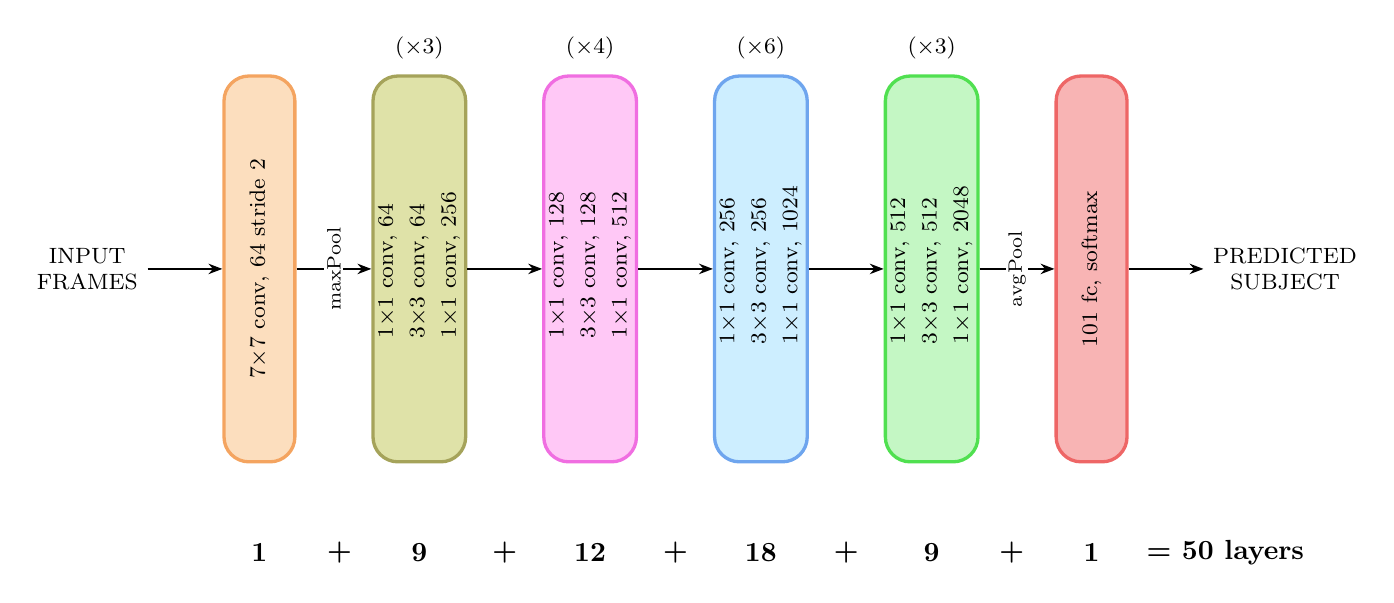
\begin{tikzpicture}[
                pill/.style={draw, rounded corners=9pt, very thick, minimum height=4.9cm, minimum width=0.9cm, inner sep=2pt, font=\footnotesize},
                io/.style={align=center, font=\footnotesize},
                arrow/.style={-{Stealth[length=5pt]}, thick},
                lab/.style={rotate=90, font=\scriptsize, fill=white, inner sep=1pt},
                cnt/.style={font=\footnotesize, above=2pt},
                node distance=0.95cm]
            \definecolor{cstem}{RGB}{252,222,190}\definecolor{bstem}{RGB}{244,164,96}
            \definecolor{c1}{RGB}{223,226,168}\definecolor{b1}{RGB}{165,163,90}
            \definecolor{c2}{RGB}{255,200,246}\definecolor{b2}{RGB}{240,110,225}
            \definecolor{c3}{RGB}{205,238,255}\definecolor{b3}{RGB}{110,165,238}
            \definecolor{c4}{RGB}{196,247,196}\definecolor{b4}{RGB}{80,224,80}
            \definecolor{cfc}{RGB}{248,180,180}\definecolor{bfc}{RGB}{238,102,102}
            \node[io] (in) {INPUT\\FRAMES};
            \node[pill, fill=cstem, draw=bstem, right=of in] (stem) {\rotatebox{90}{7$\times$7 conv, 64 stride 2}};
            \node[pill, fill=c1, draw=b1, right=of stem] (l1) {\begin{tabular}{@{}c@{\hspace{0.55em}}c@{\hspace{0.55em}}c@{}}\rotatebox{90}{1$\times$1 conv, 64} & \rotatebox{90}{3$\times$3 conv, 64} & \rotatebox{90}{1$\times$1 conv, 256}\end{tabular}};
            \node[pill, fill=c2, draw=b2, right=of l1] (l2) {\begin{tabular}{@{}c@{\hspace{0.55em}}c@{\hspace{0.55em}}c@{}}\rotatebox{90}{1$\times$1 conv, 128} & \rotatebox{90}{3$\times$3 conv, 128} & \rotatebox{90}{1$\times$1 conv, 512}\end{tabular}};
            \node[pill, fill=c3, draw=b3, right=of l2] (l3) {\begin{tabular}{@{}c@{\hspace{0.55em}}c@{\hspace{0.55em}}c@{}}\rotatebox{90}{1$\times$1 conv, 256} & \rotatebox{90}{3$\times$3 conv, 256} & \rotatebox{90}{1$\times$1 conv, 1024}\end{tabular}};
            \node[pill, fill=c4, draw=b4, right=of l3] (l4) {\begin{tabular}{@{}c@{\hspace{0.55em}}c@{\hspace{0.55em}}c@{}}\rotatebox{90}{1$\times$1 conv, 512} & \rotatebox{90}{3$\times$3 conv, 512} & \rotatebox{90}{1$\times$1 conv, 2048}\end{tabular}};
            \node[pill, fill=cfc, draw=bfc, right=of l4] (fc) {\rotatebox{90}{101 fc, softmax}};
            \node[io, right=of fc] (out) {PREDICTED\\SUBJECT};
            \draw[arrow] (in) -- (stem);
            \draw[arrow] (stem) -- (l1) node[midway, lab] {maxPool};
            \draw[arrow] (l1) -- (l2);
            \draw[arrow] (l2) -- (l3);
            \draw[arrow] (l3) -- (l4);
            \draw[arrow] (l4) -- (fc) node[midway, lab] {avgPool};
            \draw[arrow] (fc) -- (out);
            \node[cnt] at (l1.north) {($\times$3)};
            \node[cnt] at (l2.north) {($\times$4)};
            \node[cnt] at (l3.north) {($\times$6)};
            \node[cnt] at (l4.north) {($\times$3)};
            \node[font=\bfseries\normalsize, below=0.9cm of stem] (c0) {1};
            \node[font=\bfseries\normalsize, below=0.9cm of l1] (c1n) {9};
            \node[font=\bfseries\normalsize, below=0.9cm of l2] (c2n) {12};
            \node[font=\bfseries\normalsize, below=0.9cm of l3] (c3n) {18};
            \node[font=\bfseries\normalsize, below=0.9cm of l4] (c4n) {9};
            \node[font=\bfseries\normalsize, below=0.9cm of fc] (c5n) {1};
            \foreach \a/\b in {c0/c1n, c1n/c2n, c2n/c3n, c3n/c4n, c4n/c5n} \node[font=\bfseries\normalsize] at ($(\a)!0.5!(\b)$) {+};
            \node[font=\bfseries\normalsize, right=0.35cm of c5n] {= 50 layers};
        \end{tikzpicture}
    \end{adjustbox}
    \caption{Kiến trúc ResNet-50: mỗi hộp là một stage, ghi các convolution của một bottleneck block và số lần lặp (\(\times n\)); hàng dưới đếm số layer có trọng số của từng phần. Ở chế độ partial, stem, stage 1 và stage 2 (hộp thứ nhất đến thứ ba) bị đóng băng; classification head có 101 đầu ra.}
    \label{fig:a1-resnet}
\end{figure}

Các layer này được ghép thành \emph{bottleneck block} (Hình~\ref{fig:a1-block}): convolution \(1\times1\) đầu giảm số kênh (ví dụ 256 xuống 64) để convolution \(3\times3\) giảm khối lượng tính toán, rồi convolution \(1\times1\) cuối tăng lại gấp 4; ở block đầu mỗi stage, residual connection dùng thêm một convolution \(1\times1\) (\emph{projection shortcut}) để khớp kích thước.

\begin{figure}[!htb]
    \centering
    \begin{adjustbox}{max width=\linewidth}
        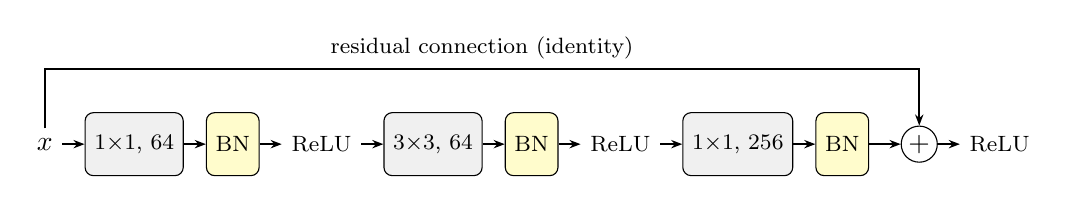
\begin{tikzpicture}[
                op/.style={draw, rounded corners=3pt, minimum height=0.8cm, font=\footnotesize, fill=black!6, align=center},
                bn/.style={draw, rounded corners=3pt, minimum height=0.8cm, font=\footnotesize, fill=yellow!20},
                act/.style={font=\footnotesize},
                arrow/.style={-{Stealth[length=4pt]}, thick},
                node distance=0.28cm]
            \node (x) {\(x\)};
            \node[op, right=of x] (c1) {\(1{\times}1\), 64};
            \node[bn, right=of c1] (b1) {BN};
            \node[act, right=of b1] (r1) {ReLU};
            \node[op, right=of r1] (c2) {\(3{\times}3\), 64};
            \node[bn, right=of c2] (b2) {BN};
            \node[act, right=of b2] (r2) {ReLU};
            \node[op, right=of r2] (c3) {\(1{\times}1\), 256};
            \node[bn, right=of c3] (b3) {BN};
            \node[draw, circle, inner sep=1pt, right=0.4cm of b3] (add) {\(+\)};
            \node[act, right=of add] (r3) {ReLU};
            \foreach \a/\b in {x/c1, c1/b1, b1/r1, r1/c2, c2/b2, b2/r2, r2/c3, c3/b3, b3/add, add/r3} \draw[arrow] (\a) -- (\b);
            \draw[arrow] (x.north) -- ++(0,0.75) -| node[near start, above, font=\footnotesize] {residual connection (identity)} (add.north);
        \end{tikzpicture}
    \end{adjustbox}
    \caption{Bottleneck block của ResNet-50 (ví dụ block thứ hai của stage 1, \(x\) có 256 kênh): ba convolution, mỗi convolution theo sau là BatchNorm (BN); đầu vào \(x\) được cộng vào đầu ra trước ReLU cuối. Ở block đầu của mỗi stage, nhánh residual connection là một convolution \(1{\times}1\) kèm BatchNorm thay cho phép chép nguyên (identity).}
    \label{fig:a1-block}
\end{figure}

\FloatBarrier

\subsubsection{DeiT-S}\label{sec:a1-deit}
DeiT-S (\emph{Data-efficient image Transformer}, bản small) là một Vision Transformer~\cite{dosovitskiy2021vit} cỡ nhỏ~\cite{touvron2021deit}: 12 Transformer block, mỗi token 384 chiều, multi-head self-attention 6 head. Điểm mới của DeiT là cách huấn luyện giúp Transformer đạt accuracy tốt khi chỉ train trên ImageNet-1k. Ảnh \(224\times224\) được chia thành 196 patch \(16\times16\), mỗi patch được chiếu thành một token 384 chiều (\emph{patch embedding}); thêm class token (CLS) và positional embedding, chuỗi 197 token đi qua 12 Transformer block với kích thước không đổi; cuối cùng class token qua LayerNorm và một fully connected layer cho ra 101 điểm số.

Các layer trong DeiT-S và chức năng của chúng:
\begin{itemize}
    \item \textbf{Patch embedding:} một convolution \(16\times16\) stride 16, tương đương một linear projection, biến mỗi patch thành một vector 384 chiều (một token).
    \item \textbf{Class token (CLS) và positional embedding:} class token là một vector học được, thêm vào đầu chuỗi để gom thông tin của cả ảnh cho bước phân loại; positional embedding cộng vào từng token để mô hình biết mỗi patch nằm ở đâu.
    \item \textbf{Layer normalization (LayerNorm):} chuẩn hoá từng token theo chính các giá trị của token đó, không phụ thuộc batch.
    \item \textbf{Multi-head self-attention:} gồm ba linear layer tạo query, key và value cho mỗi token, và một linear layer chiếu kết quả về 384 chiều. Nó cho mỗi token lấy thông tin từ mọi token khác, với trọng số tuỳ mức độ liên quan; nhờ vậy một patch nhìn được toàn ảnh ngay từ block đầu. 6 head chạy song song, mỗi head có thể chú ý đến một kiểu quan hệ khác nhau.
    \item \textbf{MLP:} hai linear layer (384 lên 1536 rồi về 384) với activation function GELU, một phiên bản mềm của ReLU, xử lý riêng từng token.
    \item \textbf{Residual connection:} như ở ResNet-50, cộng đầu vào của mỗi phần vào đầu ra của nó.
    \item \textbf{Fully connected layer và softmax:} biến class token thành 101 điểm số (logit) rồi thành xác suất.
\end{itemize}

Các layer này được ghép thành \emph{Transformer block} (Hình~\ref{fig:a1-deit-block}): multi-head self-attention rồi MLP, mỗi phần có LayerNorm đứng trước và một residual connection.

\begin{figure}[!htb]
    \centering
    \begin{adjustbox}{max width=\linewidth}
        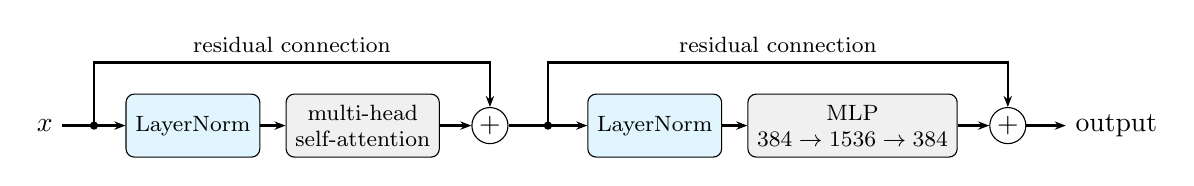
\begin{tikzpicture}[
                op/.style={draw, rounded corners=3pt, minimum height=0.8cm, font=\footnotesize, fill=black!6, align=center},
                ln/.style={draw, rounded corners=3pt, minimum height=0.8cm, font=\footnotesize, fill=cyan!12},
                arrow/.style={-{Stealth[length=4pt]}, thick},
                node distance=0.32cm]
            \node (x) {\(x\)};
            \node[ln, right=0.8cm of x] (n1) {LayerNorm};
            \node[op, right=of n1] (att) {multi-head\\self-attention};
            \node[draw, circle, inner sep=1pt, right=0.4cm of att] (a1) {\(+\)};
            \node[ln, right=1.0cm of a1] (n2) {LayerNorm};
            \node[op, right=of n2] (mlp) {MLP\\\(384\to1536\to384\)};
            \node[draw, circle, inner sep=1pt, right=0.4cm of mlp] (a2) {\(+\)};
            \node[right=0.5cm of a2] (y) {output};
            \coordinate (b1) at ($(x.east)!0.5!(n1.west)$);
            \coordinate (b2) at ($(a1.east)!0.5!(n2.west)$);
            \draw[arrow] (x) -- (n1);
            \draw[arrow] (n1) -- (att);
            \draw[arrow] (att) -- (a1);
            \draw[arrow] (a1) -- (n2);
            \draw[arrow] (n2) -- (mlp);
            \draw[arrow] (mlp) -- (a2);
            \draw[arrow] (a2) -- (y);
            \fill (b1) circle (1.5pt);
            \fill (b2) circle (1.5pt);
            \draw[arrow] (b1) -- ++(0,0.8) -| node[near start, above, font=\footnotesize] {residual connection} (a1.north);
            \draw[arrow] (b2) -- ++(0,0.8) -| node[near start, above, font=\footnotesize] {residual connection} (a2.north);
        \end{tikzpicture}
    \end{adjustbox}
    \caption{Một Transformer block của DeiT-S (\(x\) là chuỗi 197 token \(\times\) 384): LayerNorm đứng trước multi-head self-attention và MLP, và đầu vào của mỗi phần được cộng vào đầu ra của nó (residual connection).}
    \label{fig:a1-deit-block}
\end{figure}

\FloatBarrier

\subsection{Các chế độ đóng băng}\label{sec:a1-modes}
Mỗi mô hình được huấn luyện theo bốn chế độ, khác nhau ở trọng số khởi tạo và phần mạng được cập nhật (Bảng~\ref{tab:a1-modes}). Hai mô hình nhân bốn chế độ thành 8 run, mỗi run train một lần với seed 42 trên toàn bộ tập train; dữ liệu, split, hàm loss và loại optimizer (AdamW) giống nhau ở cả bốn chế độ, còn learning rate, số epoch, warmup và dropout khác nhau theo chế độ (Mục~\ref{sec:a1-hparams}).

\begin{table}[!htbp]
    \centering
    \small
    \begin{adjustbox}{max width=\linewidth}
        \begin{tabular}{lllrrr}
            \toprule
            Chế độ  & Khởi tạo   & Phần được học           & Epoch dự tính & ResNet-50 trainable   & DeiT-S trainable      \\
            \midrule
            scratch & ngẫu nhiên & toàn bộ mạng            & 100           & 23\,714\,981 (100\%)  & 21\,704\,549 (100\%)  \\
            head    & pretrained & chỉ classification head & 100           & 206\,949 (0.9\%)      & 38\,885 (0.2\%)       \\
            partial & pretrained & nửa sau của mạng        & 100           & 22\,270\,053 (93.9\%) & 10\,686\,437 (49.2\%) \\
            full    & pretrained & toàn bộ mạng            & 100           & 23\,714\,981 (100\%)  & 21\,704\,549 (100\%)  \\
            \bottomrule
        \end{tabular}
    \end{adjustbox}
    \caption{Bốn chế độ huấn luyện, số epoch dự tính và số tham số được học.}
    \label{tab:a1-modes}
\end{table}

\textbf{Scratch (train từ đầu).} Mô hình khởi tạo ngẫu nhiên, không dùng trọng số pretrained, và mọi tham số đều được học. Đây là mốc cho biết mô hình học được gì chỉ từ khoảng 68\,000 ảnh Food-101, và dùng để đo pretrain giúp được bao nhiêu. Mọi chế độ dùng cùng số epoch tối đa (100) và early stopping quyết định thời điểm dừng; scratch thường chạy lâu nhất vì phải học mọi thứ từ đầu.

\textbf{Head (chỉ train classification head).} Mô hình nạp trọng số pretrained ImageNet-1k, classification head được thay bằng một linear layer 101 đầu ra khởi tạo ngẫu nhiên, và \emph{chỉ layer này được học}; mọi phần còn lại bị đóng băng. Mô hình dùng nguyên các đặc trưng đã học từ ImageNet và chỉ học cách đọc chúng cho 101 món, nên chỉ có 0.9\% (ResNet-50) và 0.2\% (DeiT-S) số tham số được cập nhật. Đây là chế độ rẻ nhất và cho biết các đặc trưng pretrained đã tốt đến đâu với Food-101.

\textbf{Partial (đóng băng nửa đầu).} Mô hình nạp trọng số pretrained, nửa đầu của mạng (tính theo độ sâu) bị đóng băng, còn nửa sau và classification head được học. Nửa đầu giữ các đặc trưng cấp thấp như cạnh và kết cấu; nửa sau được điều chỉnh cho món ăn. Với ResNet-50, phần đóng băng gồm stem, stage 1 và stage 2; với DeiT-S, gồm patch embedding, class token, positional embedding và 6 Transformer block đầu. Vì ResNet-50 dồn tham số ở hai stage cuối còn 12 block của DeiT-S có cùng kích thước, cùng là nửa đầu nhưng ResNet-50 vẫn học 93.9\% tham số còn DeiT-S học 49.2\%.

\textbf{Full (finetune toàn bộ).} Mô hình nạp trọng số pretrained rồi cập nhật \emph{mọi} tham số với learning rate nhỏ, nên các đặc trưng pretrained được điều chỉnh dần cho Food-101. Đây là cách dùng thông dụng nhất của pretrain và thường cho accuracy cao, với chi phí tính toán bằng chế độ scratch trên mỗi epoch nhưng thường hội tụ sau ít epoch hơn scratch.

\FloatBarrier

\subsection{Siêu tham số huấn luyện}\label{sec:a1-hparams}
Cả 8 run dùng chung một công thức; chỉ learning rate, warmup và dropout đổi theo chế độ. Mọi giá trị nằm trong Bảng~\ref{tab:a1-hparams} và giống nhau ở ResNet-50 và DeiT-S.

\begin{table}[!htbp]
    \centering
    \small
    \begin{tabular}{lrrrr}
        \toprule
        Tham số & scratch & head & partial & full \\
        \midrule
        Optimizer & \multicolumn{4}{c}{AdamW, weight decay 0.05} \\
        Hàm loss & \multicolumn{4}{c}{cross-entropy, label smoothing 0.2} \\
        Lịch learning rate & \multicolumn{4}{c}{warmup tuyến tính rồi cosine về 0, cập nhật mỗi iteration} \\
        Batch (train / đánh giá) & \multicolumn{4}{c}{128 / 256} \\
        Độ chính xác số, seed & \multicolumn{4}{c}{bf16 autocast, seed 42} \\
        Epoch tối đa & \multicolumn{4}{c}{100} \\
        Early stopping (patience) & \multicolumn{4}{c}{10 epoch theo validation accuracy} \\
        \midrule
        Learning rate & $5\times10^{-4}$ & $1\times10^{-3}$ & $2\times10^{-4}$ & $1\times10^{-4}$ \\
        Warmup (epoch) & 5 & 1 & 1 & 1 \\
        Dropout (trước lớp phân loại) & 0.4 & 0.2 & 0.3 & 0.4 \\
        \bottomrule
    \end{tabular}
    \caption{Siêu tham số. Ba dòng cuối khác nhau theo chế độ. Patience là số epoch liên tiếp không có validation accuracy tốt hơn mà run còn chịu được; checkpoint giữ lại luôn là epoch có validation accuracy cao nhất, nên 100 là số epoch tối đa. Dropout đặt trên đặc trưng đã gộp ngay trước lớp phân loại cuối, cùng một vị trí ở hai kiến trúc. Weight decay không áp dụng cho bias, scale của lớp chuẩn hoá, class token và positional embedding.}
    \label{tab:a1-hparams}
\end{table}

Lý do các tham số khác nhau giữa các chế độ:
\begin{itemize}
    \item \textbf{Learning rate} giảm dần theo số trọng số pretrained được cập nhật: head ($10^{-3}$) chỉ học một lớp tuyến tính khởi tạo ngẫu nhiên nên chịu được bước lớn; partial và full ($2\times10^{-4}$ và $10^{-4}$) cập nhật cả các trọng số đã học tốt từ ImageNet nên cần bước nhỏ để không phá chúng. Scratch ($5\times10^{-4}$) khởi tạo ngẫu nhiên toàn bộ nên dùng giá trị lớn hơn.
    \item \textbf{Warmup} dài hơn ở scratch (5 epoch so với 1): khi mọi trọng số đều ngẫu nhiên, vài bước đầu với learning rate lớn dễ làm huấn luyện bất ổn, nhất là với Transformer.
    \item \textbf{Dropout} tăng theo số trọng số được học: 0.2 ở head, 0.3 ở partial, 0.4 ở full và scratch.
\end{itemize}

\subsection{Độ đo đánh giá}\label{sec:a1-eval}
Cả 8 run được đánh giá theo cùng một quy trình:
\begin{itemize}
    \item \textbf{Chọn checkpoint:} giữ epoch có validation accuracy cao nhất, rồi chấm checkpoint đó một lần trên test. Test không dùng cho bất kỳ quyết định nào.
    \item \textbf{Chất lượng:} test accuracy là chỉ số chính; kèm macro precision, recall, F1 và accuracy từng lớp.
    \item \textbf{Chi phí:} số tham số được học, thời gian mỗi epoch, bộ nhớ GPU đỉnh và tốc độ suy luận.
    \item \textbf{Phân tích lỗi:} confusion matrix, các cặp lớp bị nhầm nhiều nhất và các ảnh sai với độ tự tin cao, trên mô hình CNN và Transformer tốt nhất theo validation.
    \item \textbf{Các so sánh:} DeiT-S với ResNet-50 trong từng chế độ; full với scratch (pretrain giúp bao nhiêu); head và partial với full (mất bao nhiêu khi đóng băng); chi phí đặt cạnh accuracy.
\end{itemize}

\section{Kết quả và phân tích}\label{sec:a1-results}\label{sec:a1-analysis}
Mục này đọc tám run (2 mô hình với 4 chế độ mỗi mô hình). Mỗi cấu hình được train một lần với seed 42. Checkpoint đem ra test là epoch có validation accuracy cao nhất, và test không tham gia chọn epoch, mô hình hay siêu tham số. Chỉ số chính là test accuracy trên 25\,250 ảnh.

Trong cùng một chế độ, ResNet-50 và DeiT-S dùng chung tập ảnh, pipeline, hàm loss, AdamW, learning rate, warmup và dropout. Validation và test luôn cố định, nên mọi run được chấm trên đúng cùng các ảnh.

%-------------------------------------------------------------------
\subsection{Độ chính xác}\label{sec:a1-accuracy}
Bảng~\ref{tab:a1-results} gồm accuracy, F1 và chi phí của 8 run; Bảng~\ref{tab:a1-metrics} gồm precision, recall và F1 macro; Bảng~\ref{tab:a1-diffs} cho thấy test accuracy thay đổi bao nhiêu khi đổi chế độ.

\aonetable{results_a1.tex}{Kết quả của 8 run: số tham số được học, validation và test accuracy, F1 macro, thời gian mỗi epoch, bộ nhớ GPU đỉnh và tốc độ suy luận trên GPU A10G. In đậm: giá trị tốt nhất của mỗi cột (accuracy, F1 và img/s cao nhất; s/epoch và GB thấp nhất).}{tab:a1-results}{scripts/a1/analyze.py}

\aonetable{metrics_a1.tex}{Accuracy, precision, recall và F1 macro (trung bình trên 101 lớp) trên test. In đậm: giá trị cao nhất của mỗi cột.}{tab:a1-metrics}{scripts/a1/metrics_report.py}

\begin{table}[!htbp]
    \centering
    \small
    \setlength{\tabcolsep}{5pt}
    \begin{adjustbox}{max width=\linewidth}
        \begin{tabular}{@{}llrrrrrr@{}}
            \toprule
            & & \multicolumn{3}{c}{ResNet-50} & \multicolumn{3}{c}{DeiT-S} \\
            \cmidrule(lr){3-5}\cmidrule(l){6-8}
            Nội dung so sánh & Chuyển chế độ & Từ & Đến & Thay đổi & Từ & Đến & Thay đổi \\
            \midrule
            Pretrain giúp được bao nhiêu            & scratch \(\to\) full    & 75.5 & 81.8 & \textbf{+6.3}  & 47.7 & 83.5 & \textbf{+35.8} \\
            Chỉ train head mất bao nhiêu            & full \(\to\) head       & 81.8 & 66.7 & \textbf{\(-\)15.1} & 83.5 & 66.3 & \textbf{\(-\)17.2} \\
            Đóng băng nửa đầu mất bao nhiêu         & full \(\to\) partial    & 81.8 & 81.7 & \textbf{\(-\)0.1}  & 83.5 & 83.6 & \textbf{+0.1}  \\
            \bottomrule
        \end{tabular}
    \end{adjustbox}
    \caption{Test accuracy (\%) khi chuyển từ chế độ này sang chế độ khác. ``Từ'' và ``Đến'' lấy từ Bảng~\ref{tab:a1-results}; ``Thay đổi'' là hiệu của hai số đó, tính bằng điểm phần trăm.}
    \label{tab:a1-diffs}
\end{table}
\FloatBarrier

Trên test, DeiT-S partial đạt 83.6\% và DeiT-S full đạt 83.5\%. Hai run ResNet-50 tương ứng đạt 81.7\% và 81.8\%. Thấp nhất là DeiT-S scratch, 47.7\%. Macro precision, recall và F1 của mỗi run đều sát test accuracy của run đó (ví dụ DeiT-S head: accuracy 66.3\%, precision 67.9\%, F1 65.9\%) và giữ nguyên thứ tự này, nên accuracy mô tả được chất lượng trên cả 101 lớp. Test accuracy luôn cao hơn validation accuracy ở cả tám run (ví dụ DeiT-S partial: 79.5\% trên validation, 83.6\% trên test); một lý do có thể là validation lấy từ train còn nhiễu hơn test (Mục~\ref{sec:a1-split}).

\textbf{Hai họ trong cùng một chế độ.} Khi finetune, DeiT-S đạt 83.5\% ở full và 83.6\% ở partial, cao hơn ResNet-50 (81.8\% và 81.7\%). Ở chế độ head, DeiT-S đạt 66.3\% và ResNet-50 đạt 66.7\%, dù DeiT-S chỉ học 38\,885 tham số còn ResNet-50 học 206\,949. Khi train từ đầu, ResNet-50 đạt 75.5\% còn DeiT-S chỉ đạt 47.7\%; đây là khoảng cách lớn nhất giữa hai họ.

\textbf{Pretrain.} So với scratch, full tăng test accuracy từ 47.7\% lên 83.5\% ở DeiT-S và từ 75.5\% lên 81.8\% ở ResNet-50. DeiT-S phụ thuộc vào trọng số pretrained nhiều hơn ResNet-50. Một cách giải thích thường gặp: phép tích chập vốn chỉ nhìn vùng ảnh lân cận và dùng cùng một filter ở mọi vị trí, nên ResNet-50 đã có sẵn hai giả định hợp với ảnh (đặc trưng nằm ở vùng gần nhau, và một vật ở đâu trong ảnh cũng nhận ra như nhau). DeiT-S không có hai giả định này mà phải học từ dữ liệu, nên cần nhiều ảnh hơn; 68\,175 ảnh là ít đối với một Transformer.

\textbf{Đóng băng so với full.} Chỉ train head làm test accuracy giảm từ 81.8\% xuống 66.7\% ở ResNet-50 và từ 83.5\% xuống 66.3\% ở DeiT-S. Giữ nguyên đặc trưng ImageNet và chỉ học lớp phân loại chưa đủ cho 101 món. Partial và full gần như ngang nhau ở cả hai mô hình (81.7\% so với 81.8\% ở ResNet-50, 83.6\% so với 83.5\% ở DeiT-S).

%-------------------------------------------------------------------
\subsection{Quá trình huấn luyện và chi phí}\label{sec:a1-curves}\label{sec:a1-overfit}\label{sec:a1-cost}\label{sec:a1-costan}

\aonefigure{curves_a1.png}{1.0}{Validation accuracy theo epoch của 8 run. Mỗi đường kết thúc ở epoch run dừng do early stopping.}{fig:a1-curves}{scripts/a1/analyze.py}

\begin{table}[!htbp]
    \centering
    \small
    \begin{tabular}{llrrrr}
        \toprule
        Mô hình   & Chế độ  & Epoch tốt nhất & Epoch dừng & Train (\%) & Val (\%) \\
        \midrule
        ResNet-50 & scratch & 85             & 97         & 99.8       & 70.7 \\
        ResNet-50 & head    & 57             & 68         & 66.3       & 62.7 \\
        ResNet-50 & partial & 19             & 30         & 92.3       & 77.1 \\
        ResNet-50 & full    & 43             & 54         & 94.7       & 77.5 \\
        DeiT-S    & scratch & 30             & 41         & 67.4       & 43.6 \\
        DeiT-S    & head    & 9              & 20         & 63.2       & 62.5 \\
        DeiT-S    & partial & 10             & 21         & 93.3       & 79.5 \\
        DeiT-S    & full    & 15             & 26         & 95.6       & 79.4 \\
        \bottomrule
    \end{tabular}
    \caption{Epoch có validation accuracy cao nhất, epoch run dừng (epoch tốt nhất cộng 11, vì run dừng khi số epoch liên tiếp không cải thiện vượt patience 10; riêng ResNet-50 scratch cộng 12 vì được chạy làm hai đợt), và accuracy trên train và validation (Val) ở epoch tốt nhất.}
    \label{tab:a1-epochs}\label{tab:a1-gap}
\end{table}
\FloatBarrier

Hình~\ref{fig:a1-curves} và Bảng~\ref{tab:a1-epochs} cho thấy quá trình huấn luyện của 8 run. DeiT-S scratch đạt validation cao nhất ở epoch 30, rồi đi ngang quanh 41--43\% và dừng ở epoch 41. Train accuracy tại epoch đó chỉ 67.4\%. ResNet-50 scratch tiếp tục tăng validation đến epoch 85. Tại đó train accuracy là 99.8\% còn validation là 70.7\%.

Ở chế độ head, train và validation đều nằm trong khoảng 62--67\% (DeiT-S: 63.2\% và 62.5\%; ResNet-50: 66.3\% và 62.7\%). Một lớp tuyến tính không đủ sức đưa accuracy lên mức của partial và full. Partial và full khớp tập train ở mức 92--96\%, với validation 77--80\%. Partial khớp tập train ít hơn full (ResNet-50 từ 94.7\% xuống 92.3\%, DeiT-S từ 95.6\% xuống 93.3\%) trong khi validation gần như giữ nguyên; một khả năng là phần đầu mạng không được cập nhật nên mô hình bớt khớp tập train.

\aonefigure{cost_a1.png}{0.72}{Test accuracy theo tổng thời gian các bước cập nhật (phút, GPU A10G, bf16). Thời gian này không gồm lượt chấm validation.}{fig:a1-cost}{scripts/a1/analyze.py}
\FloatBarrier

Chi phí nằm ở các cột cuối của Bảng~\ref{tab:a1-results} và ở Hình~\ref{fig:a1-cost}. So với full, partial rẻ hơn mà accuracy không giảm:
\begin{itemize}
    \item \textbf{Thời gian mỗi epoch:} ResNet-50 từ 98\,s xuống 55\,s; DeiT-S từ 84\,s xuống 56\,s.
    \item \textbf{Bộ nhớ GPU đỉnh:} ResNet-50 từ 5.7\,GB xuống 1.9\,GB; DeiT-S từ 4.9\,GB xuống 2.6\,GB.
    \item \textbf{Tổng thời gian train đến khi dừng:} ResNet-50 từ 88 phút xuống 28 phút; DeiT-S từ 37 phút xuống 20 phút.
\end{itemize}
Tốn nhất là train từ đầu, ví dụ ResNet-50 scratch mất 160 phút. Khi suy luận, DeiT-S xử lý khoảng 2\,860 ảnh/giây, ResNet-50 khoảng 2\,280 ảnh/giây, tức DeiT-S nhanh hơn khoảng 25\%.

%-------------------------------------------------------------------
\subsection{Phân tích lỗi}\label{sec:a1-errors}\label{sec:a1-agreement}
Phần này dùng mô hình validation cao nhất của mỗi họ, ResNet-50 full và DeiT-S partial.

\begin{figure}[!htbp]
    \centering
    \IfFileExists{\aoneasset{confusion_resnet50_full.png}}{\includegraphics[width=0.49\linewidth]{\aoneasset{confusion_resnet50_full.png}}}{\aonemissing{confusion_resnet50_full.png}{}}
    \hfill
    \IfFileExists{\aoneasset{confusion_deit_s_partial.png}}{\includegraphics[width=0.49\linewidth]{\aoneasset{confusion_deit_s_partial.png}}}{\aonemissing{confusion_deit_s_partial.png}{}}
    \caption{Ma trận nhầm lẫn trên test (hàng là nhãn thật, cột là nhãn đoán). Trái: ResNet-50 full. Phải: DeiT-S partial.}\label{fig:a1-confusion}
\end{figure}

\begin{figure}[!htbp]
    \centering
    \IfFileExists{\aoneasset{confused_resnet50_full.png}}{\includegraphics[width=0.49\linewidth]{\aoneasset{confused_resnet50_full.png}}}{\aonemissing{confused_resnet50_full.png}{}}
    \hfill
    \IfFileExists{\aoneasset{confused_deit_s_partial.png}}{\includegraphics[width=0.49\linewidth]{\aoneasset{confused_deit_s_partial.png}}}{\aonemissing{confused_deit_s_partial.png}{}}
    \caption{15 cặp lớp bị nhầm nhiều nhất (nhãn thật $\to$ nhãn đoán) trên test. Trái: ResNet-50 full. Phải: DeiT-S partial.}\label{fig:a1-confused}
\end{figure}

\aonefigure{errors_deit_s_partial.png}{1.0}{18 ảnh test bị DeiT-S partial đoán sai với độ tự tin cao nhất (nhãn thật $\to$ nhãn đoán, xác suất trong ngoặc).}{fig:a1-errors}{scripts/a1/analyze.py}
\FloatBarrier

Ma trận đầy đủ ở Hình~\ref{fig:a1-confusion}. Hai mô hình nhầm các món trông gần nhau (Hình~\ref{fig:a1-confused}): \texttt{filet\_mignon} với \texttt{steak}, \texttt{chocolate\_cake} với \texttt{chocolate\_mousse}, \texttt{pork\_chop} với \texttt{steak}, \texttt{beef\_tartare} với \texttt{tuna\_tartare}. DeiT-S partial đoán \texttt{tuna\_tartare} thành \texttt{beef\_tartare} ở 60 trên 250 ảnh của lớp. Lớp dễ nhất với cả hai mô hình là \texttt{edamame} (99.6\% ở ResNet-50 full, 100\% ở DeiT-S partial); tiếp theo là \texttt{pad\_thai} và \texttt{macarons} ở ResNet-50, \texttt{macarons} và \texttt{pho} ở DeiT-S. Khó nhất với ResNet-50 full là \texttt{steak}, \texttt{pork\_chop} và \texttt{bread\_pudding} (51.6--58.0\%); với DeiT-S partial là \texttt{pork\_chop}, \texttt{huevos\_rancheros} và \texttt{tuna\_tartare} (54.0--57.2\%). Trong 18 ảnh sai với xác suất cao nhất (Hình~\ref{fig:a1-errors}) có cả ảnh nhiều món hoặc nhãn khó đọc, và cả lỗi thật như \texttt{hamburger} bị đoán thành \texttt{falafel}.

\aonetable{agreement_a1.tex}{ResNet-50 so với DeiT-S trên cùng 25\,250 ảnh test (\%, trừ Jaccard). Jaccard lỗi: số ảnh cả hai cùng sai chia cho số ảnh có ít nhất một mô hình sai.}{tab:a1-agreement}{scripts/a1/agreement.py}
\FloatBarrier

Ở partial và full, khoảng 10\% ảnh bị cả hai cùng sai, 6.3--6.4\% chỉ ResNet-50 đúng và 8.1--8.2\% chỉ DeiT-S đúng (Bảng~\ref{tab:a1-agreement}); Jaccard lỗi là 0.41.

%-------------------------------------------------------------------
\subsection{Giải thích dự đoán của mô hình}\label{sec:a1-explain}
ResNet-50 dùng Grad-CAM trên stage cuối. DeiT-S dùng attention rollout, không phụ thuộc lớp được đoán. Hai hình dưới dùng chung 8 ảnh test.

\aonefigure{explain_resnet50.png}{0.85}{Grad-CAM của bốn chế độ ResNet-50 trên 8 ảnh test.}{fig:a1-explain-resnet}{scripts/a1/explain.py}

\aonefigure{explain_deit_s.png}{0.85}{Attention rollout của bốn chế độ DeiT-S trên cùng 8 ảnh.}{fig:a1-explain-deit}{scripts/a1/explain.py}

\aonetable{explain_deletion.tex}{Phép xoá trên 2\,000 ảnh test: accuracy (\%) khi giữ nguyên ảnh, và khi xoá 25\% hoặc 50\% số ô theo thứ tự của bản đồ giải thích (nổi bật) hoặc ngẫu nhiên.}{tab:a1-deletion}{scripts/a1/explain.py}
\FloatBarrier

Ở partial và full, vùng nóng của cả hai mô hình nằm trên món (Hình~\ref{fig:a1-explain-resnet} và~\ref{fig:a1-explain-deit}). ResNet-50 head loang hơn, có ảnh rơi vào đĩa hoặc góc ảnh. DeiT-S scratch chỉ còn vài đốm ở rìa. Phép xoá trên 2\,000 ảnh kiểm tra bản đồ này (Bảng~\ref{tab:a1-deletion}): xoá 25\% ô nổi bật làm ResNet-50 full còn 40.0\%, xoá ngẫu nhiên còn 70.8\%. DeiT-S full còn 71.2\% và 77.6\%. Ở head, đường xoá theo rollout của DeiT-S gần như trùng đường xoá ngẫu nhiên. Xoá ngẫu nhiên 50\% ô, DeiT-S partial và full còn 72.4\% và 66.1\%, ResNet-50 partial và full còn 50.1\% và 35.4\%.

%-------------------------------------------------------------------
\FloatBarrier

\section{Thảo luận, kết luận và hạn chế}\label{sec:a1-discussion}

\subsection{Kết luận chính}\label{sec:a1-answers}\label{sec:a1-cnn-vit}\label{sec:a1-pretrain}\label{sec:a1-freeze}
\begin{itemize}
    \item \textbf{DeiT-S tốt hơn ResNet-50 khi finetune từ ImageNet, còn ResNet-50 tốt hơn khi train từ đầu.} Khi finetune, DeiT-S đạt 83.5--83.6\% test accuracy, ResNet-50 đạt 81.7--81.8\% (Mục~\ref{sec:a1-accuracy}); DeiT-S suy luận nhanh hơn khoảng 25\% (Mục~\ref{sec:a1-cost}). Khi train từ đầu, ResNet-50 đạt 75.5\%, DeiT-S chỉ đạt 47.7\%.
    \item \textbf{Transformer cần pretrain trên tập cỡ này; CNN cũng được lợi nhưng ít hơn.} Với 68\,175 ảnh train, full tăng test accuracy từ 47.7\% lên 83.5\% ở DeiT-S và từ 75.5\% lên 81.8\% ở ResNet-50.
    \item \textbf{Đóng băng nửa đầu mạng cho accuracy ngang finetune toàn bộ mà rẻ hơn; chỉ train head chỉ hợp khi thiếu tài nguyên.} Partial giảm 33--44\% thời gian mỗi epoch và 47--67\% bộ nhớ đỉnh so với full (Mục~\ref{sec:a1-cost}). Chỉ train head làm test accuracy giảm từ 81.8\% xuống 66.7\% ở ResNet-50 và từ 83.5\% xuống 66.3\% ở DeiT-S.
    \item \textbf{Hai mô hình chủ yếu nhầm các món trông giống nhau, và sai ở những ảnh khá khác nhau.} Ví dụ \texttt{steak} với \texttt{filet\_mignon}; Jaccard lỗi giữa hai mô hình là 0.41 (Mục~\ref{sec:a1-errors}).
\end{itemize}

\subsection{Hạn chế}
\begin{itemize}
    \item \textbf{Mỗi cấu hình chỉ train một lần.} Kết quả ứng với một seed duy nhất, nên các lần chạy khác có thể cho số hơi lệch.
    \item \textbf{Công thức huấn luyện chưa được tối ưu cho từng mô hình.} Hai họ dùng chung một công thức và siêu tham số được dò rất ít, nên kết quả, nhất là ở chế độ scratch, phản ánh cả công thức chứ không chỉ kiến trúc.
    \item \textbf{Mỗi họ chỉ có một mô hình.} Kết luận về CNN và Transformer chỉ chắc cho ResNet-50 và DeiT-S, chưa chắc cho các kích thước hay kiến trúc khác.
    \item \textbf{Chỉ một tập dữ liệu và một nguồn pretrain.} Food-101 có các lớp gần với ImageNet (Mục~\ref{sec:a1-reason}), nên lợi ích của pretrain có thể khác trên miền dữ liệu khác.
    \item \textbf{Phần giải thích ở quy mô nhỏ.} Grad-CAM, attention rollout và phép xoá ô chỉ dùng một tập con ảnh test và là phương pháp xấp xỉ, nên mang tính tham khảo.
    \item \textbf{Chi phí chỉ đo trên một cấu hình phần cứng.} Thời gian và bộ nhớ đo trên một GPU A10G với bf16, nên có thể khác ở phần cứng khác.
\end{itemize}

\subsection{Khả năng tái lập}
\begin{itemize}
    \item \textbf{Cấu hình tập trung.} Cấu hình của 16 run (8 train, 8 test) được sinh từ một nơi duy nhất, \texttt{scripts/\allowbreak a1/\allowbreak make\_\allowbreak configs.py}, với seed 42 và split cố định lưu thành tệp CSV.
    \item \textbf{Huấn luyện và đánh giá bằng script.} \texttt{scripts/\allowbreak train.py} huấn luyện theo từng tệp cấu hình; các script trong \texttt{scripts/\allowbreak a1/} chấm checkpoint trên test, sinh bảng, hình và các phân tích bổ sung. Mọi lựa chọn ngẫu nhiên đều có seed cố định.
    \item \textbf{Môi trường.} Các run chạy trên GPU A10G; chạy lại có thể lệch nhẹ ở chữ số thập phân của accuracy do tính không tất định của phép toán GPU và bf16.
    \item \textbf{Cách chạy lại.} Hướng dẫn từng bước nằm trong mục \emph{Chạy lại A1} của \texttt{README.md}. Checkpoint của A1 không được công bố, nên muốn có kết quả thì phải huấn luyện lại.
\end{itemize}

\addcontentsline{toc}{section}{Tài liệu}
\bibliographystyle{plain}
\bibliography{references}

\end{document}
